\section{Budgets cancellation and backpressure}\label{sec:C20:budgets}
A runtime executes under several budgets that are not interchangeable. Tokens constrain inference volume; wall-clock deadlines constrain responsiveness; tool quotas constrain access; monetary limits combine model and service costs; risk budgets constrain permitted effects. Converting all of them into one scalar can obscure hard requirements. A cheap operation may still be unauthorized, and a low-token plan may wait indefinitely on a remote tool.

Represent remaining resources by a vector $B_t$ and each candidate action by a distribution of costs. Admission requires hard constraints to hold before expected utility is considered. For a deadline $D\geq0$, current elapsed time $t\in[0,D]$, nonnegative uncertain duration $L(a)$, and tolerated miss probability $\epsilon\in(0,1)$, a chance constraint $\Pr(L(a)\leq D-t)\geq1-\epsilon$ is meaningful only when the duration model is calibrated for the workload. A mean-latency estimate does not establish a tail guarantee. Timeouts truncate observations and can bias the estimated distribution if treated as ordinary successful durations.

A hard budget also needs reservations under concurrency. For a scalar budget $B_0$, let $s_t$ be settled spend, $P_t$ outstanding operations and $r_i$ the reserved upper cost of operation $i$. Require
\begin{equation}
 s_t+\sum_{i\in P_t}r_i\leq B_0.
\end{equation}
Admission checks the invariant and reserves $r_i$ before dispatch in one linearizable budget-ledger transition. Settlement must use the same ledger and atomically add $c_i$ to settled spend while removing $r_i$ from outstanding reservations, with $0\leq c_i\leq r_i$. It is idempotent under the logical-operation key: a repeated settlement returns the recorded result without charging or releasing again. Admission, settlement and release share one serialization order. Releasing a reservation before recording its charge would let another admission consume the apparent balance and invalidate the bound. Under these assumptions, each ledger transition preserves the invariant by induction. Vector budgets use componentwise inequalities. This guarantee requires valid cost bounds and linearizable, crash-consistent accounting; an expected-cost estimate or atomic reservation alone is insufficient. Cancellation does not release a reservation until the remaining charge or effect is bounded. An unbounded remote billing path cannot be turned into a hard cap by local accounting alone.

Cancellation propagates through an ownership tree. A parent may cancel its own inference yet leave a remote command, browser navigation, or delegated worker running. The runtime needs a record of outstanding operations, cancellation support for each tool, and a reconciliation strategy for tools that cannot stop. Returning control to the user does not prove that background effects have ceased. This distinction is particularly important when a later instruction changes authorization while an earlier operation remains in flight.

Backpressure prevents an overloaded system from amplifying its own failures. If a tool slows down, retries can increase offered load and make recovery less likely. A retry policy should distinguish transport failure, rate limiting, invalid arguments, and uncertain completion. Backoff addresses congestion; it does not repair a malformed request. A circuit breaker prevents repeated calls to a failing dependency but must preserve evidence about abandoned work. Otherwise the agent may reinterpret a dependency outage as evidence that a fact or object does not exist.

The scheduling objective must also include fairness. A single long-running agent can occupy scarce browser sessions or large KV allocations while shorter requests wait. Preemption can improve fairness but increases checkpoint and reconstruction cost. The appropriate policy depends on whether progress is checkpointable and whether external operations can be safely suspended. A runtime should expose these workload properties rather than apply one universal quantum to every tool.

Benchmark admission and cancellation under open-loop arrival processes, not only fixed concurrency. Fixed concurrency reduces offered load when latency rises and can conceal instability. Report queueing delay separately from execution time, and include rejected or cancelled work in the relevant denominator. Tail latency, budget overshoot, orphaned operations, and completed useful work collectively describe whether the scheduler preserves service objectives under stress.



Figure~\ref{fig:C20:overview} isolates the mechanism and its stated information boundaries.
\begin{figure}[!htbp]
\centering
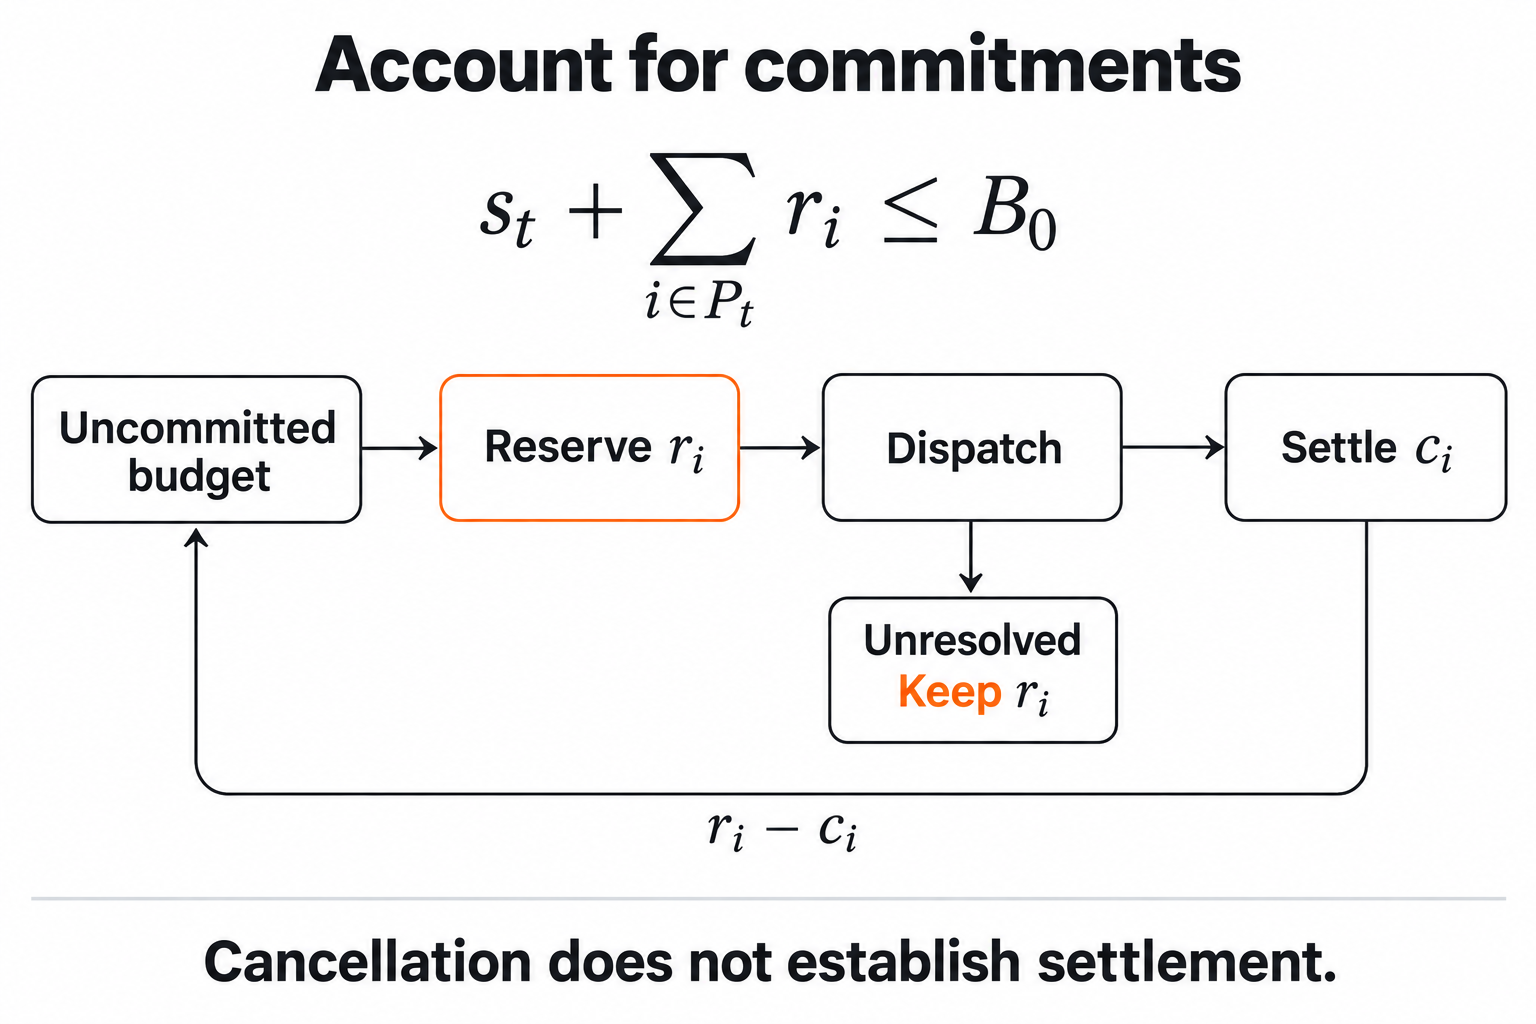
\includegraphics[width=\linewidth]{book/figures/assets/F20review.png}
\caption{A hard-budget invariant accounts for settled spend and bounded outstanding commitments. Admission reserves an upper cost before dispatch. Keyed idempotent settlement atomically records the actual charge and releases only the unused reservation in the same linearizable ledger used for admission. Unresolved operations retain commitments until remaining charges are bounded; cancellation alone does not release them.}
\label{fig:C20:overview}
\end{figure}
